\section{CỰC TRỊ CỦA HÀM SỐ}
\subsection{TÓM TẮT LÝ THUYẾT}
\subsubsection{Khái niệm cực đại, cực tiểu}
Cho hàm số $y=f(x)$ xác định, liên tục trên $(a;b)$ (có thể $a$ là $-\infty$, $b$ là $+\infty$) và $x_0\in (a;b)$:
\begin{itemize}
    \item Nếu tồn tại số $h>0$ sao cho $f(x)<f(x_0)$ với mọi $x\in \left(x_0-h;x_0+h\right)$ và $x\ne x_0$ thì ta nói hàm số $f(x)$ đạt cực đại tại điểm $x_0$.
    \item Nếu tồn tại số $h>0$ sao cho $f(x)>f(x_0)$ với mọi $x\in \left(x_0-h;x_0+h\right)$ và $x\ne x_0$ thì ta nói hàm số $f(x)$ đạt cực tiểu tại điểm $x_0$.
\end{itemize}
\begin{center}
%    \begin{tikzpicture}[scale=1, font=\footnotesize, line join=round, line cap=round, >=stealth]
%        \def\a{0.8}
%        \draw[->] (-6,0)--(1,0) node [below]{$x$};
%        \draw[->] (0,-1.5)--(0,2.5) node [right]{$y$};
%        \draw[fill] (0,0) circle(1pt) node[below left]{$O$};
%        \draw[name path={c1}]
%        (-6,2.2)..controls +(0.2:0.5) and +(110:0.2)..
%        (-4.5,1) coordinate (C);
%        \draw (-4.5,1) ..controls +(82:0.2) and +(180:0.6)..
%        (-3.5,2) coordinate[pos=.6](A);
%        \draw (-3.5,2) coordinate (D)..controls +(0:1) and +(180:1)..
%        (-1,-1) coordinate[pos=.3](B);
%        \draw (-1,-1) coordinate (E)..controls +(0:1.2) and +(70:-0.5)..
%        (1,1)
%        ;
%        \path
%        (-6,0) coordinate (M)
%        (1,0) coordinate (N)
%        ($(M)!(C)!(N)$) coordinate (C')
%        ($(M)!(D)!(N)$) coordinate (D')
%        ($(M)!(E)!(N)$) coordinate (E')
%        ($(M)!(A)!(N)$) coordinate (A')
%        ($(M)!(B)!(N)$) coordinate (B')
%        ;
%        \draw[dashed] (A)--(A') (B)--(B') (C)--(C') (D)--(D') (E)--(E');
%        \draw (-3.5-\a,2)--(-3.5+\a,2) (-1-\a,-1)--(-1+\a,-1);
%        \draw[fill] (D) circle(1pt) node[above]{\text{tiếp tuyến}};
%        \draw[fill] (A') circle(1pt) node[above right]{$a$};
%        \draw[fill] (B') circle(1pt) node[below]{$b$};
%        \draw[fill] (D') circle(1pt) node[above right]{$x_0$};
%        \draw[fill] (E') circle(1pt) node[above,text width= 0.8cm,align=justify,rectangle,draw=gray!60,rounded corners=2mm]{Điểm cực tiểu};
%        \draw[fill] (C') circle(1pt) node[below,text width= 0.75cm,align=justify,rectangle,draw=gray!60,rounded corners=2mm]{Điểm cực tiểu};
%        \draw[fill] (D') circle(1pt) node[below,text width= 0.75cm,align=justify,rectangle,draw=gray!60,rounded corners=2mm]{Điểm\\ cực đại};
%    \end{tikzpicture}
%\begin{tikzpicture}[scale=1, font=\footnotesize, line join=round, line cap=round, >=stealth]
%    \def\xmin{-2} \def\xmax{6}
%    \def\ymin{-1} \def\ymax{5}
%    \draw[->] (\xmin,0)--(\xmax,0) node [below]{$x$};
%    \draw[->] (0,\ymin)--(0,\ymax) node [left]{$y$};
%    \draw[red] (0.5,0.5) parabola bend  (1,2) (1.5,1.5)  parabola bend (2,1) (3,2.5) parabola bend (4,4) (4.5,3.5) parabola bend (5,3) (5.5,3.5)
%    (4,4)node[above]{$y=f(x)$}
%    ;
%    \draw[dashed] (1,0)--(1,2)--(0,2)
%    (2,0)--(2,1)--(0,1)
%    (4,0)--(4,4)--(0,4) (5,0)--(5,3)--(0,3);
%    \fill (1,0)circle(1pt)node[below]{$x_1$} (2,0)circle(1pt)node[below]{$x_2$}
%    (4,0)circle(1pt)node[below]{$x_3$}
%    (5,0)circle(1pt)node[below]{$x_4$}
%    (1,2)circle(1pt)
%    (2,1)circle(1pt)
%    (4,4)circle(1pt)
%    (5,3)circle(1pt)
%    (0,0)circle(1pt)node[below left]{$O$}
%    ;
%    \draw[orange,->] (2,-0.8)--(1.1,-0.4);
%    \draw[orange,->] (2,-0.8)--(3.9,-0.4);
%    \draw[blue,->] (4.5,-0.8)--(4.9,-0.4);
%    \draw[blue,->] (4.5,-0.8)--(2.1,-0.4);
%    \draw[orange,->] (-1,3)--(0,4);
%    \draw[orange,->] (-1,3)--(0,2);
%    \draw[blue,->] (-1,2)--(0,3);
%    \draw[blue,->] (-1,2)--(0,1);
%    \draw (2,-1) node{Điểm cực đại}
%    (4.5,-1) node{Điểm cực tiểu}
%    (-1.7,3.3) node{Giá trị}
%    (-1.7,2.8) node{cực đại}
%    (-1.7,2.3) node{Giá trị}
%    (-1.7,1.8) node{cực tiểu}
%    (1,-2) node{Hình 6}
%    ;
%\end{tikzpicture}
\hspace*{2cm}\begin{tikzpicture}[smooth,samples=300,scale=1.15,>=stealth]
    \draw[->,>=stealth] (-2.5,0)--(2.7,0) node[below]{$x$};
    \draw[->,>=stealth] (0,-1.5)--(0,4) node[right]{$y$};
    \draw (0,0) node[above left]{$O$};
    \draw[blue,domain=-2:2,line width = 1.2pt] plot(\x,{(\x)^3-3*(\x)+1})node[right]{$y=f(x)$};
    \draw[fill=black] (1,0) circle(1pt) (1,-1) circle(2pt) (0,-1) circle(1pt) (-1,0) circle(1pt) (-1,3) circle(2pt) (0,3) circle(1pt);
    \draw[dashed] (1,0)node[above]{\small$x_2$}--(1,-1)--(0,-1)node[left]{\small$y_2$} (-1,0)node[below]{\small$x_1$}--(-1,3)--(0,3)node[right]{\small$y_1$};

    \draw[-,dotted] (-0.5,3.7)--(4,3.7)node[right]{$(x_1;y_1)$ là điểm cực đại của đồ thị hàm số;};
    \draw[->,dotted] (-0.5,3.7)--(-1,3.15);
    \node[right] at (4.5,3.1) {$\bullet$ $x_1$ là điểm cực đại của hàm số;};
    \node[right] at (4.5,2.5) {$\bullet$ $y_1$ là giá trị cực đại của hàm số.};

    \draw[-,dotted] (2,-1)--(2,1)--(4,1)node[right]{$(x_2;y_2)$ là điểm cực tiểu của đồ thị hàm số;}; \draw[->,dotted] (2,-1)--(1.15,-1);
    \node[right] at (4.5,0.4) {$\bullet$ $x_2$ là điểm cực tiểu của hàm số;};
    \node[right] at (4.5,-0.2) {$\bullet$ $y_2$ là giá trị cực tiểu của hàm số.};
\end{tikzpicture}
%      \begin{tikzpicture}[scale=.8, font=\footnotesize, >=stealth]
%      %%Nhập giới hạn đồ thị và hàm số cần vẽ
%      \def \xmin{-3}
%      \def \xmax{3.5}
%      \def \ymin{-2.2}
%      \def \ymax{4.5}
%      %%Tự động
%      \draw[->] (\xmin,0)--(\xmax,0) node[below left] {$x$};
%      \draw[->] (0,\ymin)--(0,\ymax) node[below left] {$y$};
%      \draw[fill=black] (0,0) circle(1pt) node [below right] {$O$};
%      %%Vẽ các điểm trên 2 hệ trục
%      \draw[dashed] (0,3)--(-1,3)--(-1,0) (2,0)--(2,-1)--(0,-1);
%      \fill[black]
%      (-1,0) circle(1pt) node(C)[below,text width=0.7cm,align=flush center] {$x_{\text{CĐ}}$}
%      (0,3) circle(1pt)node(F)[right,text width=0.4cm,right,]{$y_{\text{CĐ}}$}
%      (-1,3) circle(1pt) node(G){} ++(155:2)node(G')[text width= 2cm,align=justify,rectangle,draw=gray!60,rounded corners=3mm]{Điểm cực đại của đồ thị hàm số}
%      (2,0) circle(1pt)node(A)[text width=0.7cm,above,align=center,inner sep=1pt]{$x_{\text{CT}}$}
%      (0,-1) circle(1pt)node(D)[text width=0.5cm,left,left]{$y_{\text{CT}}$}
%      (2,-1)circle(1pt)node[inner sep=1pt](E){}++(-35:2)node(E')[text width= 2.75cm,align=justify,rectangle,draw=gray!60,rounded corners=3mm]{Điểm cực tiểu của đồ thị hàm số};
%      %%Tự động
%      \begin{scope}
%          \clip (\xmin+0.01,\ymin+0.01) rectangle (\xmax-0.01,\ymax-0.01);
%          \draw[line width =1pt,samples=200,domain=\xmin+0.5:\xmax-0.01,smooth,red] plot (\x,{8/27*(\x)^3-4/9*(\x)^2-16/9*(\x)+53/27});
%      \end{scope}
%      \draw[-stealth,out=90,in=-90,inner sep=0](E'.north)to(E);
%      \draw[-stealth,out=0,in=90,inner sep=0](G'.east)to(G);
%  \end{tikzpicture}
\end{center}
\subsubsection{Các định lý cần nhớ}%[Nguyễn Văn Nay-dự án tex TL Lê Văn Đoàn]
\begin{dl} \textbf{(điều kiện cần)}\\
    Nếu hàm số $y=f(x)$ có đạo hàm trên khoảng $(a;b)$ và đạt cực đại (hoặc cực tiểu) tại $x_0$ thì $f'(x_0)=0$.
\end{dl}
\begin{dl}\textbf{(điều kiện đủ)}\\
    Giả sử $y=f(x)$ liên tục trên khoảng $K=(x_0-h;x_0+h)$ và có đạo hàm trên $K$ hoặc trên $K\setminus \{x_0\}$, với $h>0$. Khi đó
    \begin{itemize}
        \item Nếu $f'(x)>0$ trên khoảng $(x_0-h;x_0)$ và $f'(x)<0$ trên khoảng $(x_0;x_0+h)$ thì $x_0$ là một điểm cực đại của hàm số $f(x)$.
        \item Nếu $f'(x)<0$ trên khoảng $(x_0-h;x_0)$ và $f'(x)>0$ trên khoảng $(x_0;x_0+h)$ thì $x_0$ là một điểm cực tiểu của hàm số $f(x)$.
    \end{itemize}
    \begin{center}
        \begin{minipage}[b]{8cm}
            \begin{tikzpicture}
                \tkzTabInit[nocadre=false,lgt=1.2,espcl=2.5,deltacl=0.6]
                {$x$ /0.6,$f'(x)$ /0.6,$f(x)$ /2}
                {$x_0-h$,$x_0$,$x_0+h$}
                \tkzTabLine{,+,$0$,-,}
                \tkzTabVar{-/$ $, +/$y_{\text{CĐ}}$,-/$ $}
            \end{tikzpicture}
        \end{minipage}
        \begin{minipage}[b]{8cm}
            \begin{tikzpicture}
                \tkzTabInit[nocadre=false,lgt=1.2,espcl=2.5,deltacl=0.6]
                {$x$ /0.6,$f'(x)$ /0.6,$f(x)$ /2}
                {$x_0-h$,$x_0$,$x_0+h$}
                \tkzTabLine{,-,$0$,+,}
                \tkzTabVar{+/$ $, -/$y_{\text{CT}}$,+/$ $}
            \end{tikzpicture}
        \end{minipage}
    \end{center}
    \textbf{Nói cách khác}:
    \begin{itemize}
        \item Nếu $f'(x)$ đổi dấu từ \textit{âm sang dương} khi $x$ đi qua điểm $x_0$ (theo chiều tăng) thì hàm số $y=f(x)$ đạt \textit{cực tiểu} tại điểm $x_0$.
        \item Nếu $f'(x)$ đổi dấu từ \textit{dương sang âm} khi $x$ đi qua điểm $x_0$ (theo chiều tăng) thì hàm số $y=f(x)$ đạt \textit{cực đại} tại điểm $x_0$.
    \end{itemize}
\end{dl}
%\begin{dl}
%    Giả sử $y=f(x)$ có đạo hàm cấp hai trong khoảng $(x_0-h;x_0+h)$, với $h>0$. Khi đó
%    \begin{itemize}
%        \item Nếu $y'(x_0)=0$, $y''(x_0)>0$ thì $x_0$ là điểm cực tiểu.
%        \item Nếu $y'(x_0)=0$, $y''(x_0)<0$ thì $x_0$ là điểm cực đại.
%    \end{itemize}
%    \begin{nx}
%        Một hàm số chỉ có thể đạt cực trị tại một điểm mà tại đó đạo hàm của hàm số bằng $0$, hoặc tại đó hàm số không có đạo hàm, chẳng hạn hàm số $y=\left|x\right|$.
%    \end{nx}
%\end{dl}
